%\documentclass[12pt, draftclsnofoot, onecolumn,letterpaper]{IEEEtran}
\documentclass[12pt, letterpaper]{article}
%\documentclass[12pt, letterpaper]{IEEEtran}
\usepackage{ multirow }
\usepackage{longtable}
\usepackage{geometry}
\usepackage{ragged2e}
\usepackage[table]{xcolor}
\usepackage{booktabs}
\usepackage{graphicx}
\usepackage{caption}
\usepackage{subcaption}
\usepackage{lipsum}
\usepackage{makeidx}
\usepackage{enumerate}
\usepackage{color}
\usepackage{refstyle}
\usepackage{cite}
\usepackage{amsmath}
\usepackage{amssymb}
\usepackage{nomencl}
\usepackage{amsmath}
\usepackage{multirow}
\usepackage{graphicx}
\usepackage{multirow}
\usepackage{anysize}
\usepackage{float}
\usepackage{epstopdf}
\usepackage{threeparttable}
\usepackage{multicol}
\usepackage{amssymb}
\usepackage{adjustbox}
%\usepackage[none]{hyphenat}
%\usepackage{float}

%\usepackage{fixltx2e}
\usepackage{amsmath, amssymb, upgreek, amsthm}
\usepackage{graphicx}
\usepackage{tikz}
\geometry{letterpaper, left=20mm, right=20mm, top=20mm, bottom=20mm}
\usetikzlibrary{patterns} % LATEX and plain TEX when using Tik Z
\allowdisplaybreaks
\setlength{\textfloatsep}{2ex}
\usepackage{array}
\usepackage{enumitem}
\setlength{\parindent}{1 em}
\setlength{\parskip}{0.5 em}
\renewcommand{\baselinestretch}{1.25}
\def\dsd{d_\text{SD}}
\def\Rcoop{R_\text{Coop}}
\def\rhd{R_\text{HD}}
\def\rsd{R_\text{SD}}
\def\rsh{R_\text{SH}}
\def\Pcoops{\mathcal{P}^\text{Succ}_\text{Coop}}
\def\dsh{d_\text{SH}}
\def\dhd{d_\text{HD}}
\def\psibar{\overline{\mathcal{P}}^\text{Succ}_{i}}
\def\psbara{\overline{\mathcal{P}}^\text{Succ}_{1}}
\def\psbarb{\overline{\mathcal{P}}^\text{Succ}_{2}}
\def\psbarc{\overline{\mathcal{P}}^\text{Succ}_{3}}
\def\psbard{\overline{\mathcal{P}}^\text{Succ}_{4}}
\def\psbare{\overline{\mathcal{P}}^\text{Succ}_{5}}
\def\Ri{R_{i}}
\def\Ps{\mathcal{P}^\text{Succ}_\text{Direct}}
\def\frk{\mathrm{f}_{r_k}(r)}
\def\Rcoopj{R_\text{coop}^j}
\title{\bf \vspace*{-4ex} Statement of Responses to the Editor and the Reviewers of Paper-TNSM \\[-6ex]}
\date{}

\begin{document}
%\vspace*{-10ex}
%\sloppy
\maketitle
We would like to thank the editor and reviewers for their comments on our manuscript.
We hope that the modifications that we have made to the manuscript, and the responses that we have
provided herein will alleviate the reviewers' concerns. Below, please find our detailed responses to the editor and reviewers' comments and suggestions.
\\ [-3.ex]
% % % % % % % % % % % % % % % Editor % % % % % % % % % % % % % % % % % % % %


\clearpage
\noindent
\begin{longtable}{|p{0.975\textwidth}|}
\hline \hline
\Centering
\cellcolor{gray!60}
\textbf{Editor} \\
\hline \hline %\hline \hline \hline
\RaggedRight
\cellcolor{violet!15}
\textbf{\noindent Comment1:} ``The paper has gone through three independent reviews and also checked by myself. The topic is interesting and there are merits. But there are some major concerns on the contribution, the assumption, the model derivation, and the experimental results. I hope the review comments are useful for further improving the quality of the paper. I'd therefore recommend the Resubmission''\\
\hline
\end{longtable}

\vspace*{-1\baselineskip}
\noindent \textbf{Response:\\}
We would like to thank the editor for his comment on our manuscript and giving us the opportunity to resubmit it. We have utilized the comments to improve our paper and eliminate the problems.

%\begin{longtable}{|p{0.975\textwidth}|}
%\hline \hline
%\RaggedRight
%\cellcolor{green!10}
%[1] F. Patolsky, B. P. Timko, G. Yu, Y. Fang, A. B. Greytak, G. Zheng, and C. M. Lieber, ``Detection, stimulation, and inhibition of neuronal signals with high-density nanowire transistor arrays,'' Science, vol. 313, no. 5790, pp. 1100-1104, 2006.
%\\
%\hline
%\end{longtable}




% % % % % % % % % % % % % % % Reviewer 1 % % % % % % % % % % % % % % % % % % % %
\clearpage
\noindent
\begin{longtable}{|p{.975\textwidth}|}
\hline \hline %\hline \hline \hline
\Centering
\cellcolor{gray!60}
\textbf{Reviewer 1} \\
\hline \hline %\hline \hline \hline
\RaggedRight
\cellcolor{violet!15}
\textbf{\noindent Comments to the Author} ``
The paper proposes resolving the problem of resource allocation to network slices by using a new algorithm applied to the reformulation of the problem. The results seem promising but the paper has some issues. ''\\
\hline
\end{longtable}
\vspace*{-1\baselineskip}
\noindent \textbf{Response:\\}
We would like to thank the reviewer for the careful and thorough reading of this manuscript. We hope that the responses provided herein can alleviate the reviewer's concerns.

\begin{longtable}{|p{0.975\textwidth}|}
\hline \hline
\RaggedRight
\cellcolor{gray!15}
\textbf{\noindent Comment1:} ``First, the structure of the paper makes it somewhat hard to follow and there are some mistakes in the text. A proofread is required before it can be accepted for publication.   ''\\
\hline
\end{longtable}
\vspace*{-1\baselineskip}
\noindent \textbf{Response:\\}
I have changed the paper's introduction and checked the text entirely according to this comment. 





\begin{longtable}{|p{0.975\textwidth}|}
\hline \hline
\RaggedRight
\cellcolor{gray!15}
\textbf{\noindent Comment 2:} ``Although the paper demonstrates its claims, the relaxation of conditions from the original problem formulation is not well justified. It is not clear why the initial formulation of the problem is not feasible and the reformulated makes it feasible while retaining some level of quality of the solutions given. A deeper analysis of both formulations must be presented. ''\\
\hline
\end{longtable}
\vspace*{-1\baselineskip}
\noindent \textbf{Response:\\}
The problem (13) is feasible and has feasibility points that are discussed in subsection  IV-B, and we introduce a fast algorithm (algorithm 3) for feasibility points. Although the problem is feasible, it is not convex and difficult to solve.. Since problem (13) is mixed-integer nonlinear programming with two integer constraints which are a binary variable ($e$ shows the PRB assignment) and an integer variable ($M_s$ indicate the number of VNFs in slice s), the problem is NP-hard. Solving the problem is complex. To solve the problem by inspiring Stackelberg, we reformulate the equation (13g) to reduce one of the variables ($M_s$) that can be solved after obtaining the rate of UEs ($M_s$ is similar to followers in Stackelberg Competition and power and PRB assignment is similar to leader). So, the new problem has two variables of power and PRB assignment. This new problem is convex by relaxing the binary variable (PRB assignment) and estimating the lower bounds in equation (15) because the objective function and constraints of the problem are convex and can be solved by the Lagrangian function. After obtaining the power of UEs and PRB assignment, we can obtain the achievable rate of each UE so we can find the optimal number of VNFs.

We also add this response in subsection III-A.


\begin{longtable}{|p{0.975\textwidth}|}
\hline \hline
\RaggedRight
\cellcolor{gray!15}
\textbf{\noindent Comment3:} ``Moreover, the baseline and FBDR methods used in the comparison are not well introduced. They are vaguely linked to related work but not as needed. The paper must clarify the relation of the related work and the compared alternatives. The paper must also contextualize the proposal among the related work by comparing their qualities and/or performance.  ''\\
\hline
\end{longtable}
\vspace*{-1\baselineskip}
\noindent \textbf{Response:\\}
 Two different methods are used to compare with the performance of the proposed method (IABV) and show the optimality of our approach. The first one is a baseline scheme, which uses random PRB allocation. So, the allocation of PRB to each UE is random when we have low interference, but in figures with high interference, we randomly assign just one RB to each UE. Also, the association of O-RU is carried out based on distance. It means that each UE is assigned to the nearest O-RU. The optimal power is obtained using the CVX of Matlab, which uses the successive convex approximation (SCA) method since the problem is convex. 
After achieving power and other parameters, the achievable rate will be obtained and the optimal number of VNF is
achieved from the lemma (1). The second one is similar
to the fixed BBU capacity and dynamic resource allocation
(FBDR) algorithm proposed in [18]. In this work, we have services with different QoS that
contain UEs, which is similar to tenants with different QoS
that is introduced in [18]. So, we used an algorithm similar
to FBDR adapted to our conditions for comparison. Instead
of BBU in C-RAN, we have O-DU and O-CU in O-RAN.
To use the FBDR method, we should consider the fixed
BBU capacity. We assume that O-DU and O-CU have fixed
sufficient capacity in our system model. Also, our mid-haul
link (F1 link) has adequate capacity, so there will be no
issue using the FBDR method by separating BBU to O-DU
and O-CU with this assumption. In this method, PRB and power are dynamically allocated. The number of VNFs is
obtained from the simulation. The UEs are associated with the O-RU based on the quality of their channels and the
channel distance instead of using the greedy algorithm 1 (GAA algorithm ) for O-RU assignment. The figures in [18]
show that dynamic BBU capacity and dynamic resource allocation (DBDR) perform better than FBDR for the same
priority area. We will also see that our proposed algorithm performs better than FBDR in the numerical result section.


\begin{longtable}{|p{0.975\textwidth}|}
\hline \hline
\RaggedRight
\cellcolor{gray!15}
\textbf{\noindent Comment4:} ``Finally, the source of the values used for the parameters in the evaluation must be clarified.  ''\\
\hline
\end{longtable}
\vspace*{-1\baselineskip}
\noindent \textbf{Response:\\}
We refer to the following list of references in our numerical result for this comment:

\begin{longtable}{|p{0.975\textwidth}|}
\hline \hline
\RaggedRight
\cellcolor{green!10}
[1] 3GPP-TS-36.104-V13.3.0, “Evolved Universal Terrestrial Radio Access (E-UTRA);
Base Station (BS) radio transmission and reception
(Release 13),” 2016-03.

[2]  3GPP-TR-36.931-V13.0.0, “Technical Specification Group Radio Access Network;
Evolved Universal Terrestrial Radio Access (E-UTRA);
Radio Frequency (RF) requirements for LTE Pico Node B
(Release 13),” 2016-01.

[3] 3GPP-TS-25.101-V4.13.0, “User equipment (UE) radio transmission
and reception (FDD)(release 4),” 2006-12.

[4]E. Mohyeldin, “Minimum technical performance requirements for
imt-2020 radio interface(s),” 2020.

[5]  ETSI-TR-138-913-V14.3.0, “5G; study on scenarios and require-
ments for next generation access technologies(3GPP TR 38.913 version
14.3.0 release 14),” 2017-10.

\\
\hline
\end{longtable}

In [1] page 11, the amount of BW is explained. In [2], noise power is represented. In [5], the author stated the amount of delay for eMBB and URLLC in page 24 and 25. Also, in page 27, the mMTC packet size is stated. In [3], in page 13, table 6.1, the maximum power is stated. In [4], in page 4, the delay of URLLC and eMBB is stated also the spectral efficiency of eMBB is stated.
%%%%%%%%%%%%%%%%%%%%%%%%%%%%%%%%%%%%%%%%%%%%%%%%%%%%%%%%

\clearpage
\noindent
\begin{longtable}{|p{0.975\textwidth}|}
\hline \hline
\Centering
\cellcolor{gray!45}
\textbf{Reviewer 2} \\
\hline \hline
\RaggedRight
\cellcolor{violet!15}
\textbf{\noindent Comments to the Author:} ``The paper focus on the aspect of network slicing in 5G cellular network which entails a service aware resource allocation of the different required virtual network functions (VNFs) for different slices which have different characteristics. More specifically, the paper proposes a mixed integer mathematical problem which in the original form is non-linear and hence hard to solve. To tackle this challenge the optimization problem is decomposed into two sub-problems where the solutions are not optimal however numerical investigations show that the solutions are competitive. In general, the paper is well written and structured.''\\
\hline
\end{longtable}
\vspace*{-1\baselineskip}
\noindent \textbf{Response:\\}
We would like to thank the reviewer for careful and thorough reading of this manuscript and
for the thoughtful comments and constructive suggestions, which help us to improve the quality of
this manuscript. We hope that the responses provided herein can alleviate the reviewer concerns.



\begin{longtable}{|p{0.975\textwidth}|}
\hline \hline
\RaggedRight
\cellcolor{gray!15}
\textbf{\noindent Comment 2:} ``In Introduction, page 5, ``We consider a neuro-spike communication channel between two neurons located in the motor cortex region of the brain where the information is encoded by spike time intervals.''.  Please provide a reference for this sentence.''\\
\hline
\end{longtable}
\vspace*{-1\baselineskip}
\noindent \textbf{Response:\\}
Neural coding refers to the mapping from the stimulus to the configurations of the generated
spikes by neurons. Neurons employ the spike rate coding and temporal coding to transmit information via action potentials. As we explained in the manuscript, none of the papers in the literature proposed a model for neuro-spike communication channel in the motor cortex region when temporal modulations
are employed to convey information. However, there are some papers that assumed temporal modulations in the motor cortex region. We referred to one of these papers in the new manuscript based on the reviewer comment as
\begin{longtable}{|p{0.975\textwidth}|}
\hline \hline
\RaggedRight
\cellcolor{green!10}
We consider a neuro-spike communication channel between two neurons located in the motor cortex region of the brain where the information is encoded by spike time intervals [30].
\\
\hline
\end{longtable}
The referred paper is
\begin{longtable}{|p{0.975\textwidth}|}
\hline \hline
\RaggedRight
\cellcolor{green!10}
[30] Hatsopoulos N, Geman S, Amarasingham A, Bienenstock E., ``At what time scale does the nervous system operate?'', Neurocomputing, vol. 1, no. 52, pp.25-29, 2003.
\\
\hline
\end{longtable}

\clearpage
\begin{longtable}{|p{0.975\textwidth}|}
\hline \hline
\RaggedRight
\cellcolor{gray!15}
\textbf{\noindent Comment 3:} ``In System Model, the possibility of placing nano-machines in synapses located between motor cortex neurons must be proved. This action needs invasive surgeries, which cause further damage to the neurons.''\\
\hline
\end{longtable}
\vspace*{-1\baselineskip}
\noindent \textbf{Response:\\}
According to the advances in nano-technology and nano-communications, different design strategies
for intelligent nano-devices interfaced with the neuronal tissue were proposed in the literature. The
proposed system model in this manuscript is based on one of them. We clarify more about this issue in the following.
We refer to the following list of references in our explanation in this comment:

\begin{longtable}{|p{0.975\textwidth}|}
\hline \hline
\RaggedRight
\cellcolor{green!10}
[1] F. Patolsky, B. P. Timko, G. Yu, Y. Fang, A. B. Greytak, G. Zheng, and C. M. Lieber, ``Detection, stimulation, and inhibition of neuronal signals with high-density nanowire transistor arrays,'' Science, vol. 313, no. 5790, pp. 1100-1104, 2006.

[2] N. Sakai, J. Mareda, and S. Matile, ``Ion channels and pores, made from scratch,'' Molecular BioSyst., vol. 3, pp. 658-666, 2007.

[3] P. Gorostiza and E. Isacoff, ``Optical switches and triggers for the manipulation of ion channels and pores,'' Molecular BioSyst., vol. 3, pp. 686-704, 2007.

[4] Mesiti, Fabio, and Ilangko Balasingham. ``Nanomachine-to-neuron communication interfaces for neuronal stimulation at nanoscale.'', IEEE Journal on Selected Areas in Communications, vol. 31, no. 12, pp. 695-704, 2013.

[5] N. Rouach, E. Avignone, W. Même, A. Koulakoff, L. Venance, F. Blomstrand, and C. Giaume, ``Gap junctions and connexin expression in the normal and pathological central nervous system,'' Biology Cell, vol. 94, no. 7-8, pp. 457-475, 2002.

[6] J. Hjorth, K. T. Blackwell, and J. Hellgren Kotaleski, ``Gap junctions between striatal fast-spiking interneurons regulate spiking activity and synchronization as a function of cortical activity'', J. Neuroscience, vol. 29, no. 16, pp. 5276-5286, 2009.

[7] R. D. Traub, M. A. Whittington, E. H. Buhl, F. E. N. LeBeau, A. Bibbig, S. Boyd, H. Cross, and T. Baldeweg, ``A possible role for gap junctions in generation of very fast EEG oscillations preceding the onset of, and perhaps initiating, seizures,'' Epilepsia, vol. 42, no. 2, pp. 153-170, 2001.
\\
\hline
\end{longtable}


\clearpage
In [1], the authors described the successful attempt to interface nano-wire (NW) FET transistors (SiNW-neurons) with soma, dendrites and axon, allowing high precision measurement and
stimulation with an array of 50 NW connections per neuron. The synthesis of ion channels and pores, assembled artificially by chemical composition were reported in [2], whereas synthetic nano-scale actuators (nano-toggles, nano-keys and nano-tweezers) to manipulate ion channels were proposed in [3].
Hence, the advances in the molecular manipulation of the matter can allow the fabrication of bio-inspired SnM interfaces.
Upon these considerations and the available nano-technology, the authors in [4] identified a set of possible SnM interface implementations. We employed one type of these interfaces in our system model according to [4] which is denoted as Gap Junction Interface.


\textbf{Gap Junction Interface [4]}:

With gap junctions, two cellular membranes in direct contact are separated by only 3 nm and for each side, clusters of \textit{connexine} (Cx36) proteins [5], combine to form a channel with diameter 1-2 nm, the \textit{connexine}, allowing bidirectional flows of ions (currents) between cells. Synthetic connexines assembled \textit{in-situ} by SnMs could allow the opening of additional ion channels on the membrane, enhancing the neuronal activity. In the following figure [4], a sample scenario with multiple SnMs attached to the target neuron is depicted. This method is motivated and supported by neuro-scientific studies [6], [7] reporting the important role of gap junctions in \textit{oscillatory behaviors} and \textit{synchronization} phenomena between neurons.

\begin{figure}[H]
\centering
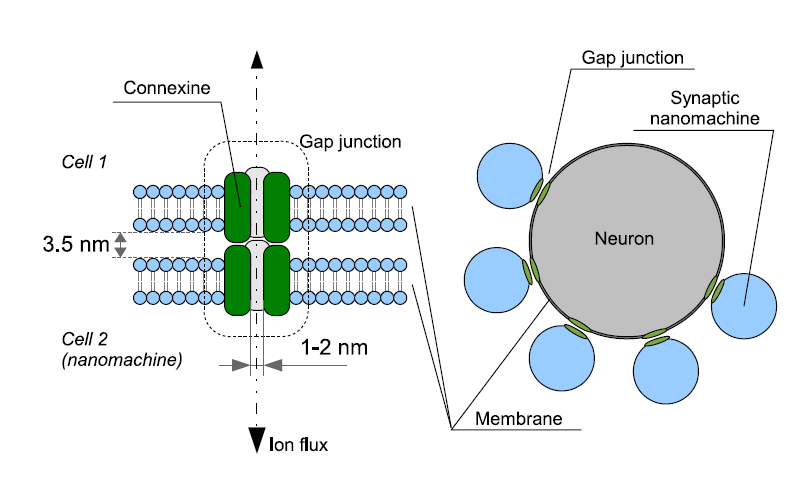
\includegraphics[width=.78\textwidth,height=.3\textheight]{Gap.png}
\caption{ Diagram of a SnM based on gap junctions. The neuronal membrane is in contact with each SnM, establishing additional connexone channels which allow the flow of ions and currents [4].}
\label{new_1}
\end{figure}


%%%%%%%%%%%%%%%%%%%%%%%%%%%%%%%%%%%%%%%%%%%%%%%%%%%%%%%%%

\clearpage
\noindent
\begin{longtable}{|p{0.975\textwidth}|}
\hline \hline
\Centering
\cellcolor{gray!45}
\textbf{Reviewer 4} \\
\hline \hline
\RaggedRight
\cellcolor{gray!15}
\textbf{\noindent Comment 1:} ``The description of  ``unhealthy neuron'' or ``neurons that have lost their ability to communicate'' and the nano-machines to connect them seems to provide a possible future application to the communication channel model proposed. What the manuscript is not fully analyzing in the opinion of this reviewer is exactly how the nano-machines could utilize this model from an engineering perspective. If this connection is not considered to be the focus and therefore was not researched, then the consideration should be made to remove the concept of nano-machines from the ``System Model'' section (and subsequent sections) and use it merely for motivating the model.''\\
\hline
\end{longtable}
\vspace*{-1\baselineskip}
\noindent \textbf{Response:\\}
We would like to thank the reviewer for careful and thorough reading of our manuscript and for
the thoughtful comments and constructive suggestions, which helped us to improve
the quality of this manuscript. We hope that the modifications that we have made to the manuscript, and the
responses that we have provided herein will alleviate the reviewer concerns.

In recent years, engineering applications of nano-technology have also been investigated with increasing interest
for the design of bio-inspired intelligent nano-devices or nano-machines connected in a network. In this manuscript, we considered the concept of nano-machines in the proposed system model according to the reported efforts to interface the neuron's body
with synthetic nano-scale materials in the literature. We provide a brief explanation in the following. We refer to the following list of references in our explanation in this comment:


\clearpage
\begin{longtable}{|p{0.975\textwidth}|}
\hline \hline
\RaggedRight
\cellcolor{green!10}
[1] F. Patolsky, B. P. Timko, G. Yu, Y. Fang, A. B. Greytak, G. Zheng, and C. M. Lieber, ``Detection, stimulation, and inhibition of neuronal signals with high-density nanowire transistor arrays,'' Science, vol. 313, no. 5790, pp. 1100-1104, 2006.

[2] N. Sakai, J. Mareda, and S. Matile, ``Ion channels and pores, made from scratch,'' Molecular BioSyst., vol. 3, pp. 658-666, 2007.

[3] P. Gorostiza and E. Isacoff, ``Optical switches and triggers for the manipulation of ion channels and pores,'' Molecular BioSyst., vol. 3, pp. 686-704, 2007.

[4] Mesiti, Fabio, and Ilangko Balasingham. ``Nanomachine-to-neuron communication interfaces for neuronal stimulation at nanoscale.'', IEEE Journal on Selected Areas in Communications, vol. 31, no. 12, pp. 695-704, 2013.

[5] N. Rouach, E. Avignone, W. Même, A. Koulakoff, L. Venance, F. Blomstrand, and C. Giaume, ``Gap junctions and connexin expression in the normal and pathological central nervous system,'' Biology Cell, vol. 94, no. 7-8, pp. 457-475, 2002.

[6] J. Hjorth, K. T. Blackwell, and J. Hellgren Kotaleski, ``Gap junctions between striatal fast-spiking interneurons regulate spiking activity and synchronization as a function of cortical activity'', J. Neuroscience, vol. 29, no. 16, pp. 5276-5286, 2009.

[7] R. D. Traub, M. A. Whittington, E. H. Buhl, F. E. N. LeBeau, A. Bibbig, S. Boyd, H. Cross, and T. Baldeweg, ``A possible role for gap junctions in generation of very fast EEG oscillations preceding the onset of, and perhaps initiating, seizures,'' Epilepsia, vol. 42, no. 2, pp. 153-170, 2001.
\\
\hline
\end{longtable}


\clearpage
In [1], the authors described the successful attempt to interface nano-wire (NW) FET transistors (SiNW-neurons) with soma, dendrites and axon, allowing high precision measurement and
stimulation with an array of 50 NW connections per neuron. The synthesis of ion channels and pores, assembled artificially by chemical composition were reported in [2], whereas synthetic nano-scale actuators (nano-toggles, nano-keys and nano-tweezers) to manipulate ion channels were proposed in [3].
Hence, the advances in the molecular manipulation of the matter can allow the fabrication of bio-inspired SnM interfaces.
Upon these considerations and the available nano-technology, the authors in [4] identified a set of possible SnM interface implementations. We employed one type of these interfaces in our system model according to [4] which is denoted as Gap Junction Interface.


\textbf{Gap Junction Interface [4]}:

With gap junctions, two cellular membranes in direct contact are separated by only 3 nm and for each side, clusters of \textit{connexine} (Cx36) proteins [5], combine to form a channel with diameter 1-2 nm, the \textit{connexine}, allowing bidirectional flows of ions (currents) between cells. Synthetic connexines assembled \textit{in-situ} by SnMs could allow the opening of additional ion channels on the membrane, enhancing the neuronal activity. In the following figure [4], a sample scenario with multiple SnMs attached to the target neuron is depicted. This method is motivated and supported by neuro-scientific studies [6], [7] reporting the important role of gap junctions in \textit{oscillatory behaviors} and \textit{synchronization} phenomena between neurons.

\begin{figure}[H]
\centering
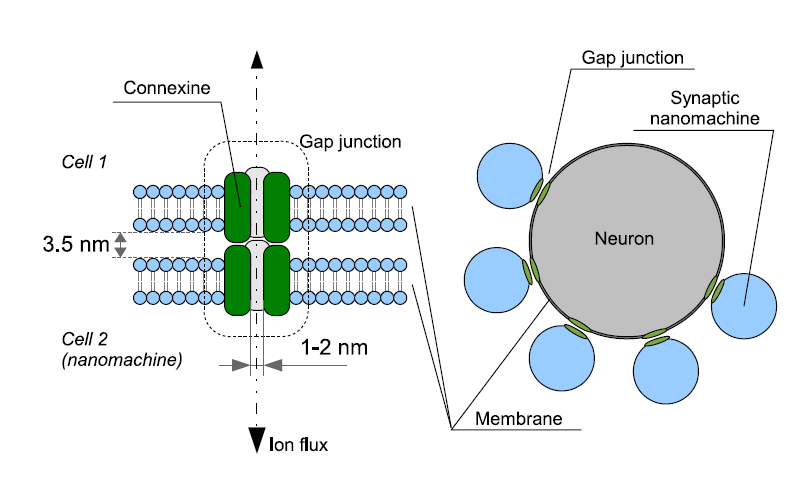
\includegraphics[width=.78\textwidth,height=.3\textheight]{Gap.png}
\caption{ Diagram of a SnM based on gap junctions. The neuronal membrane is in contact with each SnM, establishing additional connexone channels which allow the flow of ions and currents [4].}
\label{new_1}
\end{figure}










\end{document}


